\parindent=1.5em

A través de los años el hombre ha presentado un cambio radical en su nivel de vida; los conocimientos que él ha logrado acumular y aplicar han sido para su beneficio,
y han cambiado radicalmente su modo de vivir. Existe una notable diferencia entre el hombre de hace unas cuantas décadas y el hombre moderno, tal diferencia se ha
dado por el desarrollo de la ciencia, que está estrechamente relacionada con la innovacion tecnológica. Por esta razón se amplía el contenido de cómo ha
evolucionado la ciencia y la tecnología en el mundo, su origen remoto, los países que más han aportado en esta área y su respectiva utilización, bien sea para
el desarrollo o la destrucción.

Como se sabe, la tecnología se está haciendo presente en todas y cada una de las áreas de investigación, como física, química, biología, computación, y lo que es de
interés para este documento es el área de los mercados financieros.

Esta memoria está enfocada a abordar un problema financiero, relacionado con las series financieras de alta frecuencia y una forma particular
de poder realizar pronósticos tomando en cuenta distintas características de naturaleza propia de este tipo de datos. 
Se pretende abordar esta problemática con metodologías computacionales, aplicando algunos conceptos matemáticos
útiles para esta área. El problema es de carácter financiero, por lo que es necesario contextualizar el tema mediante conceptos, criterios 
y términos generales asociados al área.

Este capítulo tiene como objetivo introducir los conceptos de series de tiempo financierras, sus orígenes y la alta frecuencia.

\section{Mercados Financieros}

El mercado financiero es un espacio con marco institucional que permite poner en contacto a oferentes y demandantes para que efectúen
transacciones financieras. La idea de mercado como foro organizado a la que acuden agentes económicos para efectuar transacciones
queda reducida en el mundo financiero como las bolsas de valores.

El concepto de mercado financiero se utiliza en general para referirse a cualquier mercado organizado en el que se negocien instrumentos financieros
de todo tipo, como por ejemplo, acciones. Además, el espacio para generar estas interacciones no necesariamente debe ser físico. Por otro lado el negociar
instrumentos financieros implica a grandes rasgos: intercambiar instrumentos financieros, y definir su precio. Por ende, estos mercados están basados en
las fuerzas de oferta y demanda, ubicando a todos los oferentes en el mismo lugar para facilitarle la búsqueda a los demandantes.

Una de las razones que hace importante este tipo de mercado, es su funcionalidad, ya que permiten por un lado aumentar el capital, siendo esto uno 
de los casos favorables, ya que también hay probabilidades considerables de disminuir el capital; comercio internacional, como en los mercados de 
divisas, por ejemplo Forex; y reunir a quienes necesitan recursos financieros, con los que tienen recursos financieros. Factores claves
que permiten generar los efectos de oferta y demanda.

En este tipo de mercado se definen los siguientes términos:
\begin{itemize}
	\item \emph{Dealer}: Un dealer es un ente presente en los mercados que está dispuestos a comprar o vender.
	\item \emph{Orders}: Operación de compra/venta de activos.
	\item \emph{Bid price}: Precio al cual un \emph{dealer} está dispuesto a comprar.
	\item \emph{Ask price}: Precio al cual un \emph{dealer} está dispuesto a vender.
	\item \emph{Market orders}: instrucción del cliente al dealer, comprar o vender al mejor precio posible dentro de los valores actuales del mercado.
		Esto asegura la realización de la transacción, pero no el precio.
	\item \emph{Limit orders}: es una orden para comprar a un valor máximo (precio determinado), o para vender a un valor mínimo (precio determinado).
		Esto le da al cliente el control sobre el precio al que se ejecuta el comercio, sin embargo, no garantiza la realización de la transacción.
\end{itemize}

El conjunto de \emph{Limit orders} forman los \emph{books} para cierto activo, los cuales proveen información detallada de dicho instrumento. Con estos datos
se forman los llamados bid-ask spreads, que es la diferencia entre el precios cotizados para una venta inmediata (oferta) y una compra inmediata (bid). 
También se generan los bid-ask qoute, el cual define cotas para el precio de transacción.

\subsection{Mercados bursátiles}
Los mercados bursátiles están clasificados en los mercados de capitales, en donde se negocian activos financieros. Este tipo de mercado provee financiamiento
por medio de la emisión de acciones y permiten luego el intercambio de estas. La aplicación más directa de este tipo de mercados, son las bolsas de valores, cuyo
origen se remonta a finales del siglo XV en las ferias medievales de Europa.

Las bolsas de valores se pueden definir como mercados organizados y especializados, en los que se pueden realizar transacciones de títulos de valores por
medio de intermediarios autorizados. Estas bolsas ofrecen al público y a sus miembros facilidades, mecanismos e instrumentos técnicos que facilitan la negociación
de títulos de valores susceptibles de ofertas públicas, a precios determinados mediante subasta.

La principal función de las Bolsas de Valores implican proporcionar a los participantes información objetiva, completa y permanente de los valores
y las empresas inscritas en la bolsa, sus emisiones y las operaciones que en ella se realicen, supervisión de actividades. Las componentes de este sistema 
son los activos, instituciones financieras cuya misión es contactar demandantes y oferentes en los mercados donde se negocian
los diferentes instrumentos o activos financieros.

Dentro de los estudios de la economía, se habla de que este tipo de mercado es de competencia perfecta, ya que posee características
como: elevado número de compradores y vendedores. La decisión individual de cada uno de ellos ejercerá escasa influencia sobre el mercado global; 
Homogeneidad de los productos, es decir, no existen diferencias entre productos que venden los oferentes; Transparencia del mercado, todos los 
participantes tienen pleno conocimiento de las condiciones generales en que opera el mercado; Libertad de entrada y salida de empresas, todos 
los participantes, cuando lo deseen, podrán entrar o salir del mercado a costos nulos o casi nulos \cite{mankiw2011principles}. Sin embargo, han existido
varios estudios asociados a la Hipótesis del Mercado Eficiente, la cual dice que cuando los mercados financieros son eficientes, son capaces de trasladar 
a los precios de los activos, en cualquier momento, todos los datos relevantes de esos activos, es decir, que el precio de esos activos 
refleja en todo momento toda la información disponible sobre todos los valores y lo hace de manera insesgada. Este término lo propuso Eugene Fama en el año
1970, para y se refirió a los procesos aleatorios que se comportan como juegos justos, cuyos resultados no pueden ser predichos sistemáticamente.

\section{Series de tiempo financiera}

En la vida real, la mayoría de los fenómenos que se estudian secuencialmente, deben
tomar en cuenta la dinámica de los proceso con la finalidad tener una comprensión holística del proceso.
Una herramienta útil en dicho objetivo es el análisis de series de tiempo. Se
pueden presentar casos de series de tiempo en una multitud de disciplinas como ingeniería,
sociología, economía, finanzas por solo mencionar algunas de ellas.

El propósito fundamental es mostrar las técnicas que permitan hacer inferencias del
proceso en estudio incluyendo su predicción. Esto se logra estableciendo modelos
probabilísticos hipotéticos que representen a los datos; y en consecuencia, se lleva a cabo el
proceso de ajuste que incluye desde la estimación hasta la predicción una vez que se determina
un modelo satisfactorio. Los modelos de series deben considerar la naturaleza del fenómeno y determinar 
los factores que pueden ser incluidos en los modelos.

En particular, el análisis de una series de tiempo financiera se refiere a la teoría y práctica de la valoración 
de activos en el tiempo, intentando modelar la incertidumbre generada por las características propias del fenómeno. Tanto la teoría económica 
y sus series temporales contienen un elemento de incertidumbre. 

Las características diferenciadoras han propiciado numerosos trabajos en las áreas de econometría y economía financiera desde los años 60.
Así, en el área financiera las evidencias sobre estructuras ha conducido a la formulación de distintos modelos matemáticos que se estudiarán
en esta memoria.

\subsection{Descripción de serie financiera}

Las series de tiempo financieras como se dijo previamente, se basan en el estudio del precio de un activo financiero en el tiempo. Pero existen 
varios tipos de precios que se pueden lograr estudiar. Por un lado están los indicadores que se estudiaron en los primeros estudios formales
en esta área, llamados estudios técnicos, los cuales mostraban información al respecto de los precios: \emph{apertura}, \emph{cierre}, \emph{el más bajo}, 
\emph{el más alto}, \emph{promedio}. Esos datos lógicamente estaban orientados a tomar métricas respecto a la frecuencia \emph{día}, con estos
datos quedaban graficos como el siguiente:

\begin{center}
	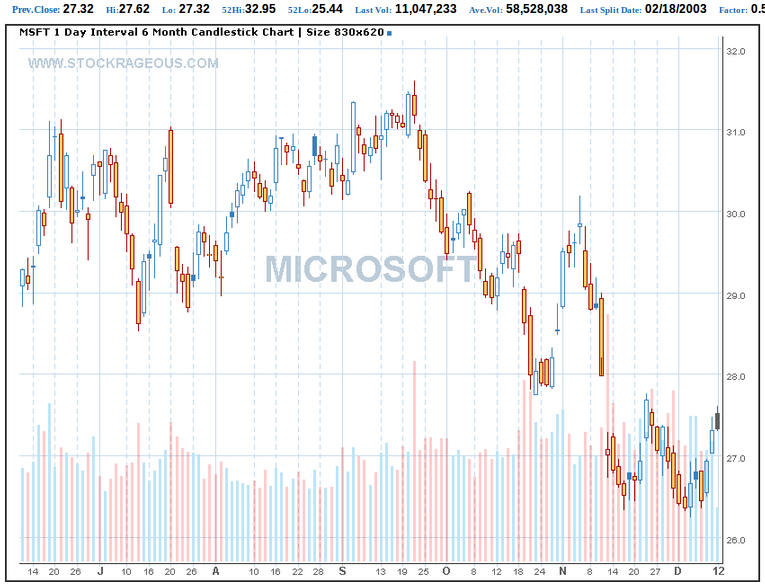
\includegraphics[width=0.6\textwidth]{images/microsoft} \\
	\textbf{Figura 1.} Información de los precios de microsoft en la bolsa. Tomada desde \url{http://www.stockrageous.com/}.
\end{center}

Esos precios son a nivel diario, ya que los estudios en esos tiempos estaban orientados a eso, como los flujos de caja, o análisis gráficos.
Sin embargo la data estudiada actualmente corresponde a data \emph{intra diaria}, la cual reside en los valores
específicos en que se compró/vendió algún activo, ya sea acción, divisa, etc. Ese término se conoce como el \emph{last price}, y corresponde
al valor específico con el cual se transó el activo. La forma de como se realiza este evento es básicamente como el que se detalló anteriormente,
es decir, mediante \emph{market} o \emph{limit orders}, por lo que existe una cola de compras/ventas obtenidas mediante los \emph{limit orders} y que cuando
se cumpla la condición asociada (de vender o comprar a cierto precio), se realiza la transacción y se registra dicho \emph{last price}; 
y por otro lado, si se entra a comprar/vender directamente mediante una \emph{market order} también se registra dicho valor. 
Juntando toda esa información entonces, se puede generar una secuencia temporal de los \emph{last prices}. Tomando en cuenta la alta frecuencia de estos datos,
se torna muy complicado manejarlo de forma humana, es por esta razón que es necesario realizar análisis cuantitativos usando computadores.

A través de la historia, estas interacciones se realizaban personalmente en las bolsas de comercio, sin embargo con el avance de las tecnologías,
se han implementado distintas plataformas de \emph{trading electrónico}: un método de negociación de valores (como acciones y bonos), divisas o derivados 
financieros por medios electrónicos. Esta tecnología de la información se utiliza para reunir a compradores y vendedores a través de la plataforma de 
comercio electrónico y las redes para crear lugares virtuales del mercado, como por ejemplo: National Association of Securities Dealers Automated 
Quotation (NASDAQ), New York Stock Exchange (NYSE), etc.

Las series financieras tienen características singulares en relación a otras series macroeconómicas, como son: 
\begin{itemize}
	\item Frecuencia: la mayor frecuencia en la observación de los datos es mayor que en otro tipo de series de tiempo, llegando incluso
		a unidades de fracciones de segundos.
	\item Heterocedasticidad: ocurre cuando la varianza de las perturbaciones no es constante a lo largo de las observaciones.
		Este factor hace inadecuados los modelos desarrolados para series estcionarias.
	\item No estacionalidad: en muchos casos presenta no estacionaridad tanto en la media como la varianza.
	\item Información oculta: se pueden encontrar distintos tipos de patrones a diferentes niveles de escala.
\end{itemize}

\subsection{High frequency trading}

Con el paso del tiempo y la implementación de distintos sistemas de trading electrónico, la frecuencia de la data creció de manera
orbitante. En estos sistemas se define un \emph{Tick}, como unidad atómica de información de un mercado financiero, particularmente sobre un activo determinado.
Esta unidad especifica una gran cantidad de parámetros como la marca temporal, precio, cantidad transada, etc. Los datos de alta frecuencia son un conjunto de datos 
de reportes detallados sobre la actividad y movimiento efectuados sobre un activo. Se reune la información de los ticks con cierto intervalo de tiempo, 
el cual para este tipo de series es variable, llegando incluso a tener ventanas de tiempo de fracciones de segundos. \emph{Wei Sun}, señala en \cite{ei2007quantitative}
que en la literatura acuñan distintos términos para referirse a este tipo de datos.

Los sistemas informáticos que realizan la labor de facilitar el comercio de instrumentos financieros, son los llamados \emph{Electronic communication networks} (ECN).
Se crearon en 1998, año que fueron autorizados por la \emph{Securities and Exchange Commission}. La SEC es una organización estadounidense que tiene la responsabilidad de
velar por el cumplimiento de las leyes federales las bolsas de valores. Esta última define formalmente el concepto de High-Frequency Trading como: \emph{} %TODO.

\section{High Performance Computing}

La capacidad de cómputo de los procesadores actuales ha incrementado de sobremanera, al igual que la cantidad de procesadores que tienen las tarjetas de video. Además, la
naturaleza de los problemas que se están estudiando, como simulación de tsunami, series de tiempo financiera, etc. Generan una gran cantidad de cómputo, por lo que es
necesario optimizar y hacer más eficientes los algoritmos. Es por esto que nace el concepto de HPC que es el área de desarrollo que aplica computadores de alto rendimiento 
(clusters) a tareas que necesitan el procesamiento eficiente de métodos complejos o de grandes volúmenes de información. La idea de base consiste en dividir los problemas 
en sub-problemas que se asignan a diferentes cores de un nodo o diferentes nodos de cálculo, coordinados por un nodo maestro mediante una red de alta velocidad. 

\section{GPU: Nvidia CUDA}
%CUDA
Las siglas GPU provienen de Graphics Processing Unit, o en español Unidad de procesamiento gráfico. Para efectos de hardware, la GPU funciona como coprocesador,
pudiéndose utilizar de forma simultánea a la CPU y así aprovechar el potencial que puedan ofrecer ambas al mismo tiempo. Una GPU es un procesador
diseñado para llevar a cabo cálculos necesarios implicados en la generación de gráficos, ya sea, para un video juego, o como para una aplicación que utilice
gráficos en 2D, o 3D. Hoy en día las GPU son muy potentes y pueden incluso superar frecuencias de reloj de una CPU antigua.

Una GPU está formada por cientos de pequeños núcleos que trabajan juntos para procesar los datos de alguna aplicación. Esta arquitectura de procesamiento paralelo
masivo es la que proporciona al GPU su alta capacidad de cálculo. Existen numerosas aplicaciones aceleradas en la GPU que brindan una forma rápida de acceder
a la computación de alto desempeño (High Performance Computing).

El concepto implícito en todo este tema es el paralelismo, que es una forma de computación en la cual varios cálculos pueden realizarse simultáneamente,
siempre y cuando no existan dependencias secuenciales entre cálculos. Basándose en "divide y vencerás", principio que busca dividir los problemas grandes, para
obtener varios problemas pequeños, que son posteriormente solucionados en paralelo.

La evolución de las tarjetas gráficas ha venido acompañado de un gran crecimiento en el mundo de los videojuegos y las aplicaciones 3D, realizándose grandes
producciones de chips gráficos por parte de grandes fabricantes, como NVIDIA, AMD (ex ATI).

En los últimos años también han aparecido conjuntos de herramientas y compiladores que facilitan la programación de las GPUs, como por ejemplo, NVIDIA CUDA, que
cuenta con la comunidad más activa hasta la fecha en programación de GPUs.

%NVIDIA CUDA
Las primeras GPU fueron diseñadas como aceleradoras de gráficos y admitían apenas procesos específicos de funcionamiento fijo. En las últimas dos decadas,
el hardware cada vez se volvió más programable, lo que culminó con la primera GPU de NVIDIA en los años 1999. En poco tiempo que se desarrollara el concepto de GPU,
investigadores empezaron a utilizar el rendimiento de estas tarjetas en cálculos con punto flotante.

Los dilemas que vivieron en futuro los programadores, fue que la programación para GPU estaba lejos de ser fácil, hasta que investigadores de la universidad de
Stanford se propusieron reimaginar la GPU como un coprocesador de flujos.

Puesto que NVIDIA sabía que su hardware era bueno e iba creciendo muy rápido, debían combinarse con herramientas de harware y software intuitivas, invitaron
a un equipo de investigación y desarrollo, para empezar a evolucionar una solución que ejecturara el lenguaje de programación C a la perfección en el GPU.
Al reunión software y hardware, NVDIA lanzó al mercado CUDA en el año 2006. La competencia AMD tuvieron intentos forzosos en generar algo similar, pero su comunidad
de desarrollo no tuvo la misma motivación que si tuvo NVIDIA CUDA.

CUDA es una plataforma de computación paralela y un modelo de programación creado por NVIDIA. La tecnología implementada por NVIDIA, es un entorno basado en el 
lenguaje C, que permite a los programadores escribir software para resolver problemas computacionales complejos en menos tiempo aprovechando la gran capacidad 
de procesamiento paralelo de las GPU multinúcleo. Miles de programadores están utilizando las herramientas gratuitas de desarrollo de CUDA (válidas para millones 
de GPU que circulan en el mercado), a fin de acelerar todo tipo de aplicaciones, desde herramientas de codificación de audio y video, diseño de productos, 
investigación científica, etc.

Actualmente NVIDIA ofrece un kit de herramientas de CUDA, las cuales incluyen un compilador, bibliotecas de matemáticas, herramientas para corregir y optimizar
redimiento de aplicaciones. Encontrándose también con muestras de código, guías de programación, manuales de usuario, referencias de la interfaz de programación
de aplicaciones (API) y otra documentación para ayudar al usuario dar los primeros pasos en el área. Cabe destacar que ofrece todo esto de forma gratuita,
incluyendo NVIDIA Parallel Nsight for Visual Studio, el primer entorno de desarrollo del sector para aplicaciones masivas paralela que usan tanto GPU como CPU, esto
en sistemas operativos Windows.

\section{Motivación}

Las características que presentan las series financieras de alta frecuencia son un problema reucrrente al querer estudiar este tipo de fenómeno. 
Estas series en la literatura se trabajan como series de tiempo, lo cual es una secuencia de observaciones ordenadas mediante índices, los cuales
son la marca temporal, información contenida en los \emph{tick}. 

El objetivo principal es diseñar e implementar un modelo de predicción considerando las características de este tipo de series, usando algoritmos de computación
de alto desempeño. Como objetivo secundarios se busca: encontrar una combinación que permita hacer más eficiente los cálculos, combinando la GPU con la CPU. 

\section{Organización de la Memoria}

Esta memoria se organizará con el siguiente esquema:
\begin{itemize}
	\item Capítulo 1: Introducción. 
	\item Capítulo 2: Estado del arte: se estudiarán y repasarán las técnicas y modelos más conocidos, distinguiendo entre modelos lineales y no lineales.
	\item Capítulo 3: Descripción formal del problema: se formalizará el problema a resolver, indicando las características consideradas.
	\item Capítulo 4: Solución propuesta: se definirá una propuesta de solución, con la respectiva metodología de implementación. 
	\item Capítulo 5: Estudio experimental: se implementará y testeará la solución propuesta, comparándola sus resultados.
	\item Capítulo 6: Conclusiones: se realizarán conclusiones generales del trabajo realizado y se detallarán posibles trabajos futuros.
\end{itemize}
